%%% The main file. It contains definitions of basic parameters and includes all other parts.

%% Settings for single-side (simplex) printing
% Margins: left 40mm, right 25mm, top and bottom 25mm
% (but beware, LaTeX adds 1in implicitly)
\documentclass[12pt,a4paper]{report}
\setlength\textwidth{145mm}
\setlength\textheight{247mm}
\setlength\oddsidemargin{15mm}
\setlength\evensidemargin{15mm}
\setlength\topmargin{0mm}
\setlength\headsep{0mm}
\setlength\headheight{0mm}
% \openright makes the following text appear on a right-hand page
\let\openright=\clearpage

%% Settings for two-sided (duplex) printing
% \documentclass[12pt,a4paper,twoside,openright]{report}
% \setlength\textwidth{145mm}
% \setlength\textheight{247mm}
% \setlength\oddsidemargin{14.2mm}
% \setlength\evensidemargin{0mm}
% \setlength\topmargin{0mm}
% \setlength\headsep{0mm}
% \setlength\headheight{0mm}
% \let\openright=\cleardoublepage

%% Generate PDF/A-2u
\usepackage[a-2u]{pdfx}

%% Character encoding: usually latin2, cp1250 or utf8:
\usepackage[utf8]{inputenc}

%% Prefer Latin Modern fonts
\usepackage{lmodern}

%% Further useful packages (included in most LaTeX distributions)
\usepackage{amsmath}        % extensions for typesetting of math
\usepackage{amsfonts}       % math fonts
\usepackage{amsthm}         % theorems, definitions, etc.
\usepackage{bbding}         % various symbols (squares, asterisks, scissors, ...)
\usepackage{bm}             % boldface symbols (\bm)
\usepackage{graphicx}       % embedding of pictures
\usepackage{fancyvrb}       % improved verbatim environment
\usepackage{natbib}         % citation style AUTHOR (YEAR), or AUTHOR [NUMBER]
\usepackage[nottoc]{tocbibind} % makes sure that bibliography and the lists
			    % of figures/tables are included in the table
			    % of contents
\usepackage{dcolumn}        % improved alignment of table columns
\usepackage{booktabs}       % improved horizontal lines in tables
\usepackage{paralist}       % improved enumerate and itemize
\usepackage{xcolor}         % typesetting in color
\usepackage[colorinlistoftodos]{todonotes} % leave in text comments
\usepackage{tipa} % use IPA characters
\usepackage[utf8]{inputenc}
\usepackage[T1]{fontenc}
\usepackage[toc, section=chapter]{glossaries}
\makeglossary

\newglossaryentry{syllable_peak}
{
	name=syllable peak,
	description={A nucleus of a syllable - either a vowel or a syllabic consonant}
}


\newglossaryentry{consonant_clusters}
{
	name=consonant cluster,
	description={A sequence of syllables without a vowel}
}

\newglossaryentry{quatrain}
{
	name=quatrain,
	description={A type of stanza consisting of four lines}
}

\newglossaryentry{LSTM}
{
	name=LSTM,
	description={Long-Sort Term Memory - a type of recurrent neural network}
}

\newglossaryentry{sonnet}
{
	name=sonnet,
	description={A poetic form traditionally containing 14 lines written in iambic pentameter with rhyme scheme \textit{abab cdcd efef gg}}
}

\newglossaryentry{headless_mode}
{
	name=headless mode,
	description={A mode in which software runs on hardware without a graphic user interface, e.g. a script in terminal}
}
\usepackage{quoting} % to indent paragraphs
\usepackage{subfig}
% To properly break urls.
%\usepackage[hyphens]{url}
\quotingsetup{leftmargin=2em, rightmargin=0in, vskip=1ex}

%%% Basic information on the thesis

% Thesis title in English (exactly as in the formal assignment)
\def\ThesisTitle{Computational analysis and synthesis of song lyrics}

% Author of the thesis
\def\ThesisAuthor{Patrícia Březinová}

% Year when the thesis is submitted
\def\YearSubmitted{2021}

% Name of the department or institute, where the work was officially assigned
% (according to the Organizational Structure of MFF UK in English,
% or a full name of a department outside MFF)
\def\Department{Institute of Formal and Applied Linguistics}

% Is it a department (katedra), or an institute (ústav)?
\def\DeptType{Institute}

% Thesis supervisor: name, surname and titles
\def\Supervisor{Mgr. Martin Popel, Ph.D.}

% Supervisor's department (again according to Organizational structure of MFF)
\def\SupervisorsDepartment{Institute of Formal and Applied Linguistics}

% Study programme and specialization
\def\StudyProgramme{Computer Science}
\def\StudyBranch{Artificial Intelligence}

% An optional dedication: you can thank whomever you wish (your supervisor,
% consultant, a person who lent the software, etc.)
\def\Dedication{%
Dedication.
}

% Abstract (recommended length around 80-200 words; this is not a copy of your thesis assignment!)
\def\Abstract{%
Abstract.
}

% 3 to 5 keywords (recommended), each enclosed in curly braces
\def\Keywords{%
{key} {words}
}

%% The hyperref package for clickable links in PDF and also for storing
%% metadata to PDF (including the table of contents).
%% Most settings are pre-set by the pdfx package.
\hypersetup{unicode}
\definecolor{dgreen}{rgb}{.0,.4,.0}
\hypersetup{
	pdfdisplaydoctitle, breaklinks,
	colorlinks,
	%pdfborderstyle={/S/U/W 1}, allbordercolors=dgreen,
	linkcolor=dgreen, citecolor=dgreen, filecolor=black, urlcolor=dgreen,
	%backref=page,
	pagebackref=true,
	pdfencoding=auto,
}


% Definitions of macros (see description inside)
%%% This file contains definitions of various useful macros and environments %%%
%%% Please add more macros here instead of cluttering other files with them. %%%

%%% Minor tweaks of style

% These macros employ a little dirty trick to convince LaTeX to typeset
% chapter headings sanely, without lots of empty space above them.
% Feel free to ignore.
\makeatletter
\def\@makechapterhead#1{
  {\parindent \z@ \raggedright \normalfont
   \Huge\bfseries \thechapter. #1
   \par\nobreak
   \vskip 20\p@
}}
\def\@makeschapterhead#1{
  {\parindent \z@ \raggedright \normalfont
   \Huge\bfseries #1
   \par\nobreak
   \vskip 20\p@
}}
\makeatother

% This macro defines a chapter, which is not numbered, but is included
% in the table of contents.
\def\chapwithtoc#1{
\chapter*{#1}
\addcontentsline{toc}{chapter}{#1}
}

% Draw black "slugs" whenever a line overflows, so that we can spot it easily.
\overfullrule=1mm

%%% Macros for definitions, theorems, claims, examples, ... (requires amsthm package)

\theoremstyle{plain}
\newtheorem{thm}{Theorem}
\newtheorem{lemma}[thm]{Lemma}
\newtheorem{claim}[thm]{Claim}

\theoremstyle{plain}
\newtheorem{defn}{Definition}

\theoremstyle{remark}
\newtheorem*{cor}{Corollary}
\newtheorem*{rem}{Remark}
\newtheorem*{example}{Example}

%%% An environment for proofs

\newenvironment{myproof}{
  \par\medskip\noindent
  \textit{Proof}.
}{
\newline
\rightline{$\qedsymbol$}
}

%%% An environment for typesetting of program code and input/output
%%% of programs. (Requires the fancyvrb package -- fancy verbatim.)

\DefineVerbatimEnvironment{code}{Verbatim}{fontsize=\small, frame=single}

%%% The field of all real and natural numbers
\newcommand{\R}{\mathbb{R}}
\newcommand{\N}{\mathbb{N}}

%%% Useful operators for statistics and probability
\DeclareMathOperator{\pr}{\textsf{P}}
\DeclareMathOperator{\E}{\textsf{E}\,}
\DeclareMathOperator{\var}{\textrm{var}}
\DeclareMathOperator{\sd}{\textrm{sd}}

%%% Transposition of a vector/matrix
\newcommand{\T}[1]{#1^\top}

%%% Various math goodies
\newcommand{\goto}{\rightarrow}
\newcommand{\gotop}{\stackrel{P}{\longrightarrow}}
\newcommand{\maon}[1]{o(n^{#1})}
\newcommand{\abs}[1]{\left|{#1}\right|}
\newcommand{\dint}{\int_0^\tau\!\!\int_0^\tau}
\newcommand{\isqr}[1]{\frac{1}{\sqrt{#1}}}

%%% Various table goodies
\newcommand{\pulrad}[1]{\raisebox{1.5ex}[0pt]{#1}}
\newcommand{\mc}[1]{\multicolumn{1}{c}{#1}}


% Title page and various mandatory informational pages
\begin{document}
%%% Title page of the thesis and other mandatory pages

%%% Title page of the thesis

\pagestyle{empty}
\hypersetup{pageanchor=false}
\begin{center}

\centerline{\mbox{
\includegraphics[width=166mm]{../img/logo-en.pdf}}}

\vspace{-8mm}
\vfill

{\bf\Large MASTER THESIS}

\vfill

{\LARGE\ThesisAuthor}

\vspace{15mm}

{\LARGE\bfseries\ThesisTitle}

\vfill

\Department

\vfill

{
\centerline{\vbox{\halign{\hbox to 0.45\hsize{\hfil #}&\hskip 0.5em\parbox[t]{0.45\hsize}{\raggedright #}\cr
Supervisor of the master thesis:&\Supervisor \cr
\noalign{\vspace{2mm}}
Study programme:&\StudyProgramme \cr
\noalign{\vspace{2mm}}
Study branch:&\StudyBranch \cr
}}}}

\vfill

% Zde doplňte rok
Prague \YearSubmitted

\end{center}

\newpage

%%% Here should be a bound sheet included -- a signed copy of the "master
%%% thesis assignment". This assignment is NOT a part of the electronic
%%% version of the thesis. DO NOT SCAN.

%%% A page with a solemn declaration to the master thesis

\openright
\hypersetup{pageanchor=true}
\pagestyle{plain}
\pagenumbering{roman}
\vglue 0pt plus 1fill

\noindent
I declare that I carried out this master thesis independently, and only with the cited
sources, literature and other professional sources. It has not been used to obtain another
or the same degree.

\medskip\noindent
I understand that my work relates to the rights and obligations under the Act No.~121/2000 Sb.,
the Copyright Act, as amended, in particular the fact that the Charles
University has the right to conclude a license agreement on the use of this
work as a school work pursuant to Section 60 subsection 1 of the Copyright~Act.

\vspace{10mm}

\hbox{\hbox to 0.5\hsize{%
In \hbox to 6em{\dotfill} date \hbox to 6em{\dotfill}
\hss}\hbox to 0.5\hsize{\dotfill\quad}}
\smallskip
\hbox{\hbox to 0.5\hsize{}\hbox to 0.5\hsize{\hfil Author's signature\hfil}}

\vspace{20mm}
\newpage

%%% Dedication

\openright

\noindent
\Dedication

\newpage

%%% Mandatory information page of the thesis

\openright

\vbox to 0.5\vsize{
\setlength\parindent{0mm}
\setlength\parskip{5mm}

Title:
\ThesisTitle

Author:
\ThesisAuthor

\DeptType:
\Department

Supervisor:
\Supervisor, \SupervisorsDepartment

Abstract:
\Abstract

Keywords:
\Keywords

\vss}

\newpage

\openright
\pagestyle{plain}
\pagenumbering{arabic}
\setcounter{page}{1}


%%% A page with automatically generated table of contents of the master thesis

\tableofcontents

%%% Each chapter is kept in a separate file
\chapter*{Introduction}
\addcontentsline{toc}{chapter}{Introduction}

As artificial intelligence keeps catching up with humans, artistic fields are still not the same without the human aspect. For computers, it is hard to create art, and even harder to understand and analyze it. 

A piece of art in everyday life of almost everyone is music. It is a complex form, where many aspects influence the audience, i.e. melody, rhythm, lyrics, performance, etc. Although we do realize they are interconnected and may affect each other, in this thesis, we will more deeply explore only one of these aspects -- song lyrics. 

We have a large crowd-sourced dataset of almost half a million song lyrics. At first, this sounded as a good base for learning a lyrics generator. However, as we explored rhymes and automatic analysis, we realized it is a much more interesting path to pursue. Every attempt at lyrics or poetry generation that we encountered used humans for their final evaluation. This proves, and \cite{greene2010automatic} agree, that automatic evaluation of poetry is hard.

Unfortunately, there was no sufficient rhyme detector that we could use for our case. In this thesis, we will dive more deeply into the problem and create one ourselves. It will give us the ability to analyze our dataset and draw interesting conclusions about the data. 

Additionally, we will create a web-page that demonstrates detector's capabilities and visualizes rhymes in an innovative way. With this tool, we hope to give artists, authors of poems and songs, or even amateurs a new way to explore their texts.

At the end, we will return to lyrics generation, that lead us down this path, and explore current state-of-art pre-trained GPT-2 and its capabilities in this field.

This works may include some literary or technical terms that the reader is not familiar with. For their definition, please see the chapter "Glossary of literary and technical terms" at the end of this thesis.


\section*{Outline}
In Chapter \ref{chap-related-work}, we will make reader familiar with the literary background such as rhyme its types, and other literary devices. We will also describe approaches and review existing tools for rhyme detection, visualization, and lyrics generation. 

Chapter \ref{data} introduces data that we will be working with, their structure and statistics, and the steps we took to pre-process them.

The most complex part of this thesis is explained in Chapter \ref{chap-rhyme-analysis}, which specifies the details of how we perform rhyme detection in song lyrics.

Chapter \ref{evaluation} evaluates our rhyme detector and shows the statistics when we run it for our dataset.

How the output of our detector is brought to life by visualization is illustrated in Chapter \ref{visualization}.

In Chapter \ref{generation}, we describe and review the results of lyrics generation experiment.

Lastly, the results are summed up in Conclusion, including suggestions for future works.
\chapter{Related work sjnkfsjndcl}


\todo[inline]{mention here rhyme generating tools like rhymezone}
\todo[inline]{Is it OK that this chapter uses IPA but IPA is explained in the next sections?}
\todo[inline]{uviest do related works aj 4 metody detekcie rymov od plechaca? ale vsetky priklady su machine learning okrem sparsaru}
\subsection{Rhyme types and literary devices}
\todo[inline]{Dat ipa s dvojteckami}
\todo[inline]{Prehodnotit definicie rymov}
Although everyone instinctively knows what a rhyme is and can recognize one in a poem or a song, it does not have a very precise definition. It is described as "a word that has the same last sound as another word" by Cambridge Dictionary (\cite{walter2008cambridge}) or a "literary device, featured particularly in poetry, in which identical or similar concluding syllables in different words are repeated" by \cite{literarydevices2020}. These definitions are not detailed enough to base a good algorithm off of, so let's look deeper into different rhyme types.

\paragraph{Perfect rhyme} (also true rhyme, or sometimes just "rhyme") is the most common and valued \todo{cite?} type of rhyme. It requires two conditions to be met:

\begin{itemize}
	\item last stressed vowel and all following sounds are identical
	\item immediately preceding sounds differ
\end{itemize}

It is also the only rhyme for which the definitions are consistent (for example, see \cite{bain1867manual}, \cite{vanphonological}, \cite{bergman2017litcharts}, \footnote{\url{https://en.wikipedia.org/wiki/Rhyme}}). It can be further distinguished depending on how many syllables are involved:

\begin{itemize}
	\item \textbf{Masculine} (also single, monosyllabic) -- "the commonest kind of rhyme, between single stressed syllables at the ends of verse" (\cite{oxforddict2008literary}). 
	Examples: 
	
	fly (\textipa{\underline{flaI}}) / sky (\textipa{\underline{skaI}})
	
	before (\textipa{bi-\underline{fOr}}) / explore (\textipa{Iks-\underline{plOr}})
	\footnote{For the examples, we are using IPA transcriptions because it is more comfortable for human reader.}
	\footnote{Stressed syllables are underlined. Syllables are separated with a hyphen.}
	
	\item \textbf{Feminine} (also double) -- "a rhyme on two syllables, the first stressed and the second unstressed" (\cite{oxforddict2008literary}). Examples: 
	
	bitten (\textipa{\underline{bI}-t@n}) / written (\textipa{\underline{rI}-t@n})
	
	lazy (\textipa{\underline{leI}-zi}) / crazy (\textipa{\underline{kreI}-zi})
	
	\item \textbf{Dactylic} (also triple) -- "a rhyme on three syllables, the first stressed and the others unstressed"(\cite{oxforddict2008literary}). Examples: 
	
	amorous (\textipa{\underline{æ}-m@r-@s}) / glamorous (\textipa{\underline{glæ}-m@r-@s})
	
	vanity (\textipa{\underline{væ}-nI-ti}) / humanity (\textipa{ju-\underline{mæ}-nI-ti}))
	
\end{itemize}

\paragraph{Imperfect rhyme} (also slant or half rhyme)  rhymes "the stressed syllable of one word with the unstressed syllable of another word" (\cite{bergman2017litcharts}). Examples: 

cabbage (\textipa{\underline{kæ}-bIdZ}) / ridge (\textipa{\underline{rIdZ}})

painting (\textipa{\underline{peI}-nIN}) / ring (\textipa{\underline{rIN}})

\noindent In other sources, definitions differ -- for example \cite{literarydevices2020} calls this effect "feminine rhyme".  On the other hand, \cite{oxforddict2008literary} and \cite{britannica} use the term "imperfect rhyme" for end-line consonance (see definition below) and \cite{vanphonological} uses it for end-line assonance (see definition below). For the purpose of this thesis we will work with the first definition mentioned.

\paragraph{Unaccented rhyme} (also weakened rhyme) "occurs when the relevant syllable of the rhyming word is unstressed" (\cite{britannica}). Examples: 

hammer (\textipa{\underline{hæ}-m@r}) / carpenter (\textipa{\underline{kAr}-p@n-t@r})

\noindent The difference opposed to imperfect rhyme is that here both rhyme fellows are unstressed.

\todo[inline]{Prehodnotit identitu}
\paragraph{Identical rhyme} (also rime riche) is "a kind of rhyme in which the rhyming elements include matching consonants before the stressed vowel sounds." This includes "rhyming of two words with the same sound and sometimes the same spelling but different meanings e.g seen (\textipa{\underline{sin})}/ scene (\textipa{\underline{sin}}). The term also covers word‐endings where the consonant preceding the stressed vowel sound is the same: compare (\textipa{k@m-\underline{pEr}}) / despair (\textipa{dI-\underline{spEr}})." (\cite{oxforddict2008literary}). It is generally considered not as good as perfect rhyme because it is too predictable for the listener\footnote{\url{https://literaryterms.net/rhyme/}}.

\paragraph{Forced rhyme} (also near rhyme) "includes words with a close but imperfect match in sound in the final syllables" \cite{bergman2017litcharts}. Examples: 

green (\textipa{\underline{grin}}) / fiend (\textipa{\underline{find}})

hide (\textipa{\underline{haId}}) / mind (\textipa{\underline{maInd}})

\noindent This includes the case when spelling in changed in order to make the rhyme work, e.g. truth (\textipa{\underline{truT}}) / endu'th (\textipa{en-\underline{duT}}) (a contraction of "endureth"). It can also refer to using unnatural word order to get the rhyming word at the end of the line (\cite{bergman2017litcharts}) but we will not make use of this interpretation in this thesis.

\paragraph{Assonance} is "repetition of stressed vowel sounds within words with different end consonants" (\cite{britannica}). Examples:	

quite (\textipa{\underline{kwaIt}}) / like (\textipa{\underline{laIk}})

free (\textipa{\underline{fri}}) / breeze (\textipa{\underline{briz}})

\noindent The term itself defines a literary device applicable anywhere in the poem but when used at the end of verse, it can sometimes be considered a rhyme (under various names) by sources like \cite{vanphonological}, \cite{bergman2017litcharts} and others.

\paragraph{Consonance} is "the recurrence or repetition of identical or similar consonants" (\cite{britannica}). Examples: 

country (\textipa{\underline{k@n}-tri}) / contra (\textipa{\underline{kAn}-tr@})

hickory dickory dock (\textipa{\underline{hI}-k@-ri \underline{dI}-k@-ri \underline{dAk}})

\noindent Similarly as assonance, it applies to repetition anywhere. When seen at the end of verse, it can be considered a rhyme and again, various terms are used, perhaps the most common is "pararhyme" (\cite{britannica}, \cite{oxforddict2008literary}).
\newline

The last two terms may seem as more of a tool for poets than songwriters. Surprisingly, they have found their way into song lyrics and have become a standard in genres like hip hop according to \cite{vanphonological}. From the creative point of view, it is not less sophisticated rather it enriches rhyme as we know it (\cite{brogan2016poeticterms}).
\todo[inline]{Mention here we're not using it as a rhyme - or maybe if it will be highlighted in the visualization?}
\todo[inline]{uviest to tam jasnejsie? definicie zo slovnikov nie su dost vyhranene (ex. consonance - nehoduju sa vowels!)
}

Other rhyme types exist e.g. eye rhyme where "the spellings of the rhyming elements match, but the sounds do not, e.g. love (\textipa{\underline{l@v}}) / prove (\textipa{\underline{pruv}})" (\cite{oxforddict2008literary}). We will be omitting them because we did not consider them relevant for song lyrics or the purpose of this thesis.

\todo[inline]{spomenut ze nevieme zistit ci to spevak nevyslovi inak ,ze moze hltat bezprizvucne slabiky viac naraz
}


\section{Rhyme detection tools}
\todo[inline]{Pridat nejaky nastroj co pouziva len CMU dictionary}
\subsection{SPARSAR}


\subsection{Unsupervised approach}
\subsubsection*{EM algorithm}
\cite{reddy2011unsupervised} proposed a language-independent model for finding rhyme schemes in poetry. They created an unsupervised model based on EM algorithm that assigns the most probable rhyme scheme for each sequence of line-final words. It achieved good results when tested on annotated English and French corpus with poetry from 15\textsuperscript{th} to 20\textsuperscript{th} century. However its big pitfall lies in the fact that it is biased towards the rhyme schemes from golden data. It has a predefined set of all rhyme schemes found in tested data and those are the only ones it chooses from. For illustration, in a 14-line stanza it can choose from 90 schemes which is only 0.00005\% of all possible options. In 29\% of cases from French corpus it has only one choice.\footnote{\url{http://versologie.cz/talks/2017basel/}}

\subsubsection*{RhymeTagger}
\cite{plechavc2018collocation} came with a collocation-driven alternative named RhymeTagger. It uses the same dataset as the previous approach with addition of a larger Czech poetry corpus\footnote{\url{https://github.com/versotym/corpusCzechVerse}}. Each line-final word is transcribed into phonetic transcription and split into components -- \gls{syllable_peak} for each syllable and \gls{consonant_clusters} in between. In the "expectation" step, probabilities for each component pair are calculated based on their co-occurrence in line-final words, e.g. conditional probability of rhyme based on peak component pair \textipa{@U:@U} will be very high but for consonant component pair k:r quite low. These statistics for component pairs are then used in the "maximization" step to calculate the probability for line-final word pair as a combined probability of all their components (paired by means of usual association measure). If the probability of two words is above a given threshold they are considered a rhyme. After all such pairs are classified, probabilities are iteratively recalculated in the EM cycle. 

For words that were not successfully classified with this method, there is a fallback. The author observed that some words are now pronounced differently than they were during the Shakespearean era they were written in and therefore using current pronunciation dictionaries may ruin the original rhyme, e.g. original near (\textipa{nE:r}) / there (\textipa{DE:r}) vs. contemporary near (\textipa{nI:r}) / there (\textipa{DE:r}). Original pronunciation can be therefore inferred from words with similar orthography. He calculated rhyme probability given final character trigrams, which helped achieve higher recall. Although other methods may have better precision, collocation-driven approach wins in recall as seen in \ref{screenshotRT}. This method does not take into account meter.

For evaluation, they used precision, recall and F-score calculated as follows:

\[PRECISION=\frac{true\ positives}{true\ positives+false\ positives}\]

\[RECALL=\frac{true\ positives}{true\ positives+false\ negatives}\]

\[F-SCORE=\frac{2*PRECISION*RECALL}{PRECISION+RECALL}\]

For an intuitive view, the reader can imagine precision as how many of algorithm's rhymes were actually rhymes and recall as how many rhymes were discovered. F-score describes the trade-off between the two.

\begin{figure}[h]\centering
	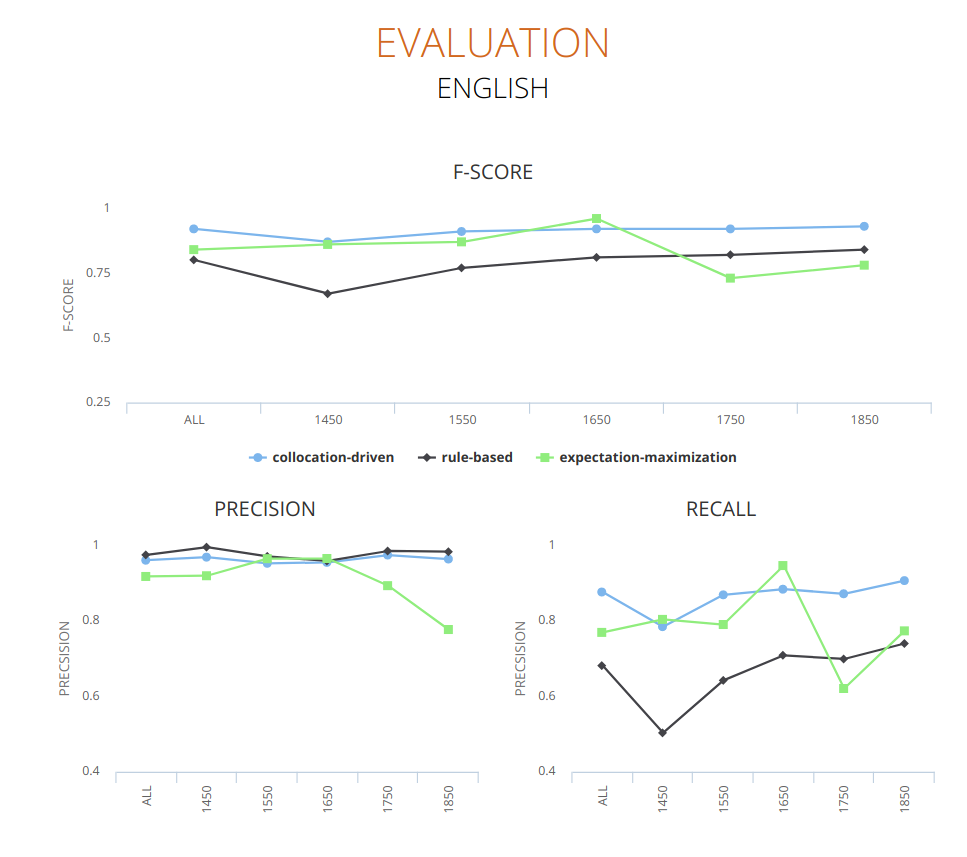
\includegraphics[scale=0.4]{../img/plechac_eval.png}
	\caption[RhymeTagger evaluation]{Evaluation of RhymeTagger on English corpus in comparison with EM algorithm and simple rule-based approach. The x axis is the year when the tested poem was written, the y axis are the evaluation scores as described above. Reproduced from \cite{plechac2017presentation}.}
	\label{screenshotRT}
\end{figure}
\todo[inline]{Popisat preco nejdu ich data pouzit na testovanie mojej detekcie rymov}

\subsubsection*{Deep-speare}
As a part of their \gls{sonnet} \gls{quatrain} generating model, \cite{lau2018deep} have implemented a Rhyme component that identifies and generates rhymes. It is a unidirectional forward \gls{LSTM} (\cite{hochreiter1997long}) that learns to separate rhyming word pairs from non-rhyming. They generate input by pairing one line-final word with the other three from the same quatrain. Since the rhyme scheme of a \gls{sonnet} \gls{quatrain} is always \textit{abab} this will result in one rhyming pair and two non-rhyming. Additional non-rhyming pairs are generated with random word sampling. Then the model with margin-based loss learns the margin separating the best pair from all the others. It returns a cosine similarity score that estimates how well do two words rhyme.

To evaluate this model, authors used phoneme matching with CMUdict \footnote{\url{http://www.speech.cs.cmu.edu/cgi-bin/cmudict}} and the EM model from \cite{reddy2011unsupervised} trained on their own data and they were able to outperform both based on F1 score.



\section{Visualization tools}
In the following section, we will describe existing visualization tools for poetry. Software mentioned below focuses on poems, however song lyrics can be considered just a more structurally relaxed version of a regular poem.
\subsection{Poem Viewer}
Quite complex and comprehensive visualization tool is Poem Viewer \cite{Abdul2013}. With no need for complicated installations it is easily available for the writers as a web-based application as shown in Figure \ref{screenshotPV}. Unfortunately, at the time of writing this thesis the upload of custom text was not working. Luckily, this is still an ongoing project so this might be just a temporary issue. Nevertheless there are some default poems available to demonstrate this software's capabilities.
\begin{figure}[h]\centering
	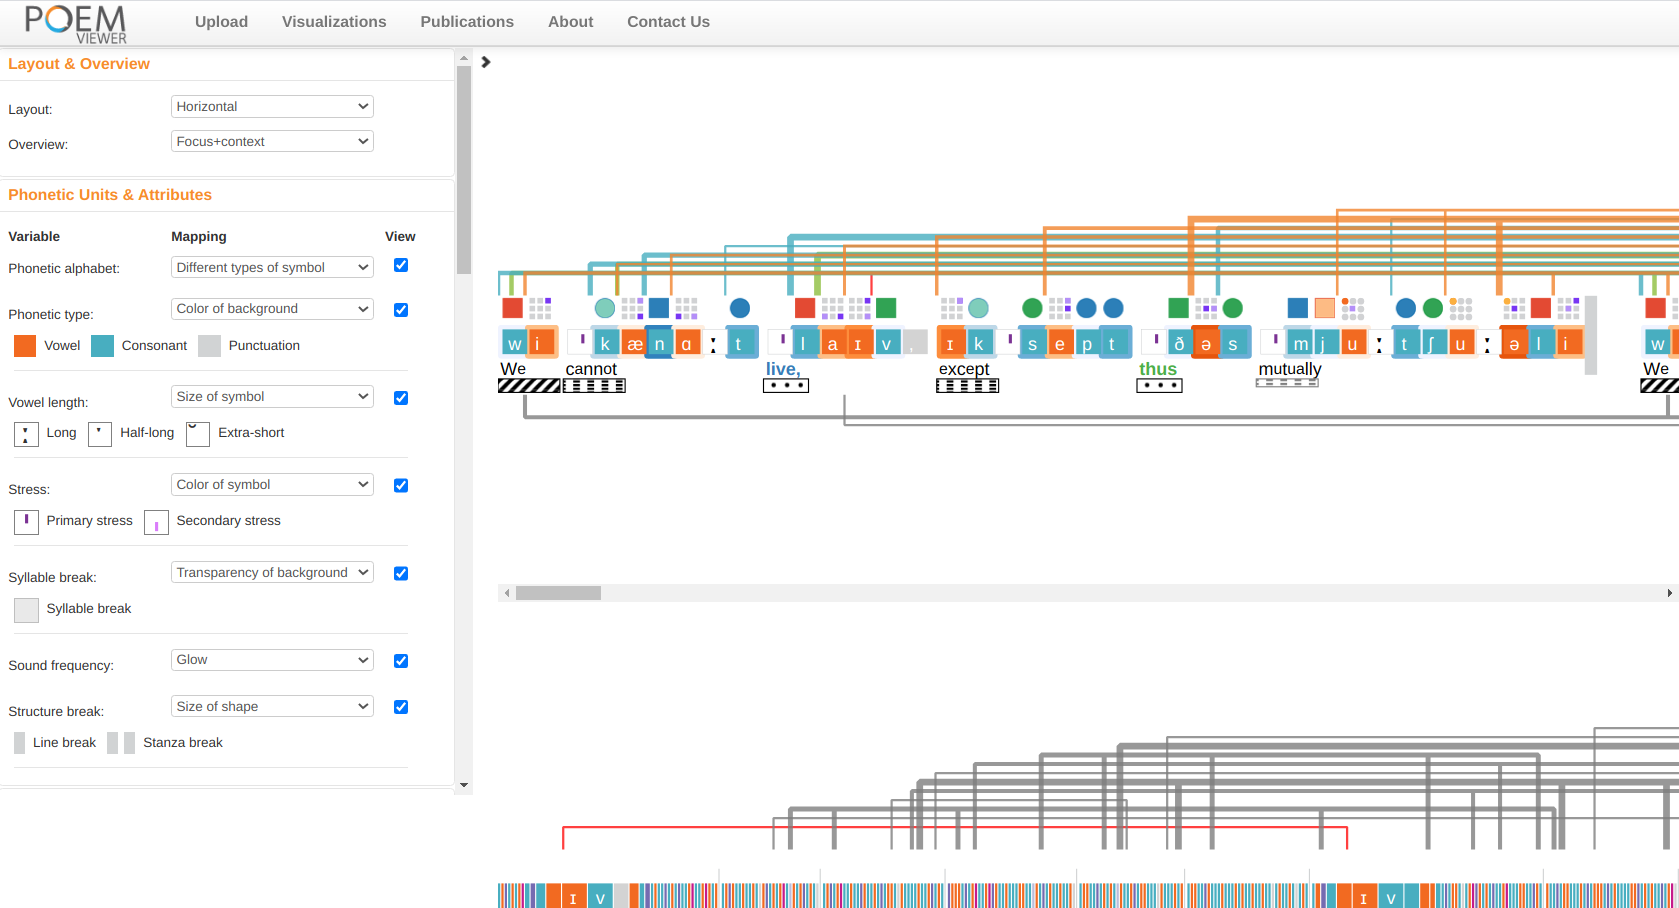
\includegraphics[scale=0.24]{../img/ScreenshotPV.png}
	\caption{Screenshot from Poem Viewer tool -- visualizing Love by Elizabeth Barrett Browning.}\label{screenshotPV}
\end{figure}

\begin{figure}[h]\centering
	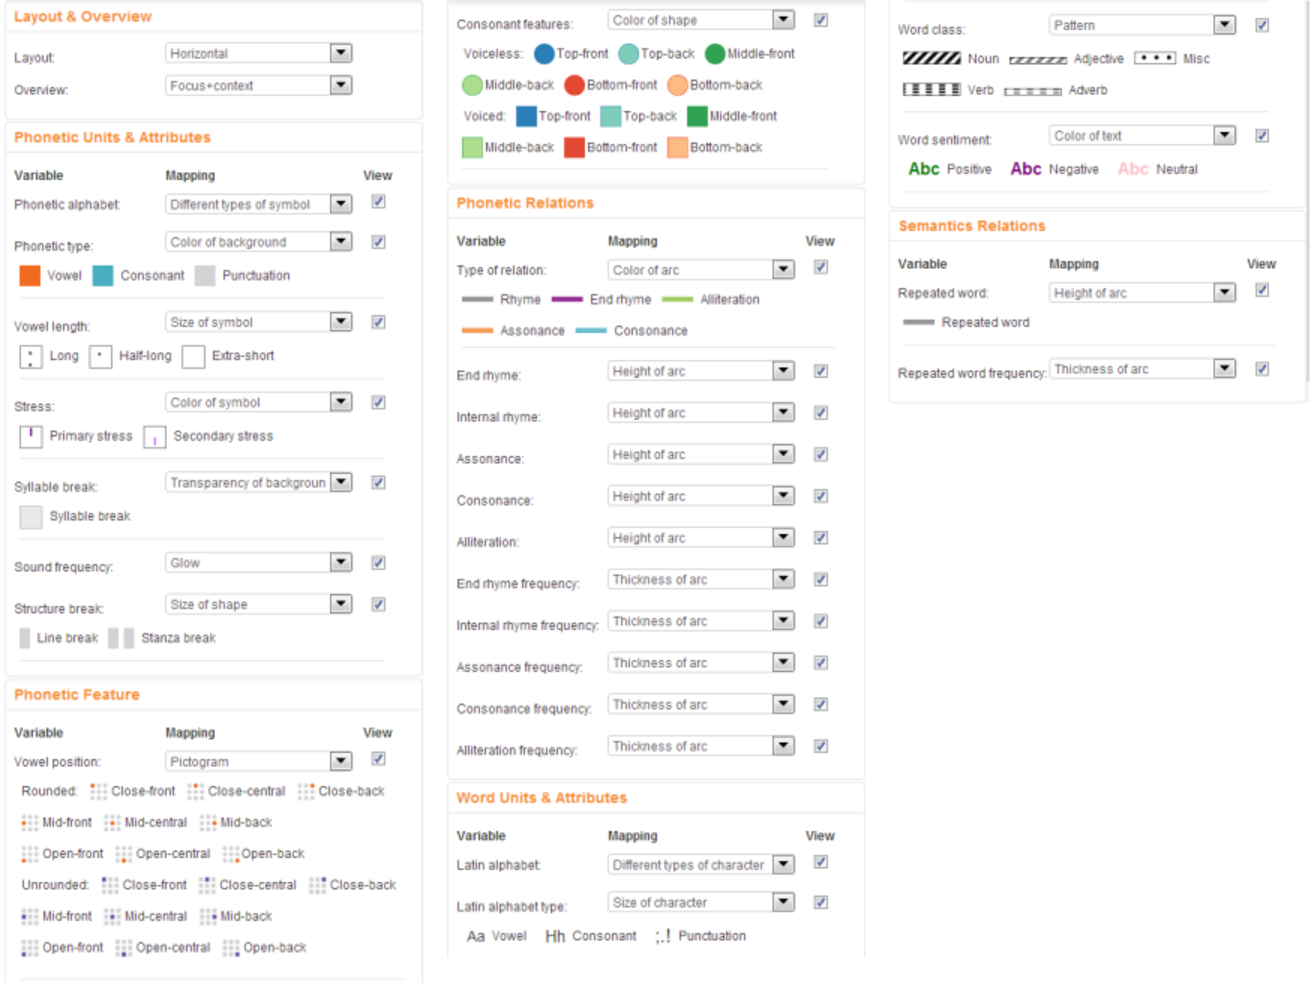
\includegraphics[scale=0.4]{../img/snapshotPV_options.pdf}
	\caption{Available options and their default mappings in Poem Viewer.}\label{screenshotPV-options}
\end{figure}

Most of the analyzed features (shown in Figure \ref{screenshotPV-options} focus on the phonetic aspects of the poem. After phonetic transcription to IPA users can analyze consonant features, vowel length and position, stress, syllables, word classes and sentiment using color codes and markers. A second layout offers six different graphs/animations of tongue positions during each verse. Arcs are used to mark end rhyme, alliteration, assonance, consonance, their particular frequencies and repeating words.


Overall this software, although very elaborate, appears crammed and confusing for an inexperienced user. Moreover, it is perhaps better suited for its original use case -- a well-structured poem -- than less regular song lyrics.

\subsection{SPARSAR}
SPARSAR (\cite{Delmonte2014}) is also a very interesting tool for poetry analysis and expressive Text-to-speech conversion. It is originally designed for a thorough examination of a very strictly structured Shakespeare's sonnets. To achieve this, it has to run analyses on many levels -- and these results can be used to analyze any poem. It looks at the poem on three levels: phonetic (pronunciation, consonant and vowel tongue position, assonances, etc.), poetic (metrical structure, rhyme schemes, acoustic length, etc.), and semantic (sentiment, methaphorically linked words, anaphora, etc.).

User can choose between a window application with graphs and diagrams or a \gls{headless_mode} with .xml output files. Its main disadvantage for our use case is that it is written in Prolog and therefore is very strict on the input format and runs only under a specific older version of Ubuntu. 

\subsection{ProseVis}
This Java desktop visualization tool by \cite{Clement2013} analyzes text through
parts-of-speech, phonemes, stress, tone, and break index. These features are extracted using OpenMary Text-to-speech system (\cite{Schroder2006}) and predictive classification. The authors believe their visualization will present the features to user in a more human readable form (\cite{prosevis2017sourceforge}).

\begin{figure}[h]\centering
	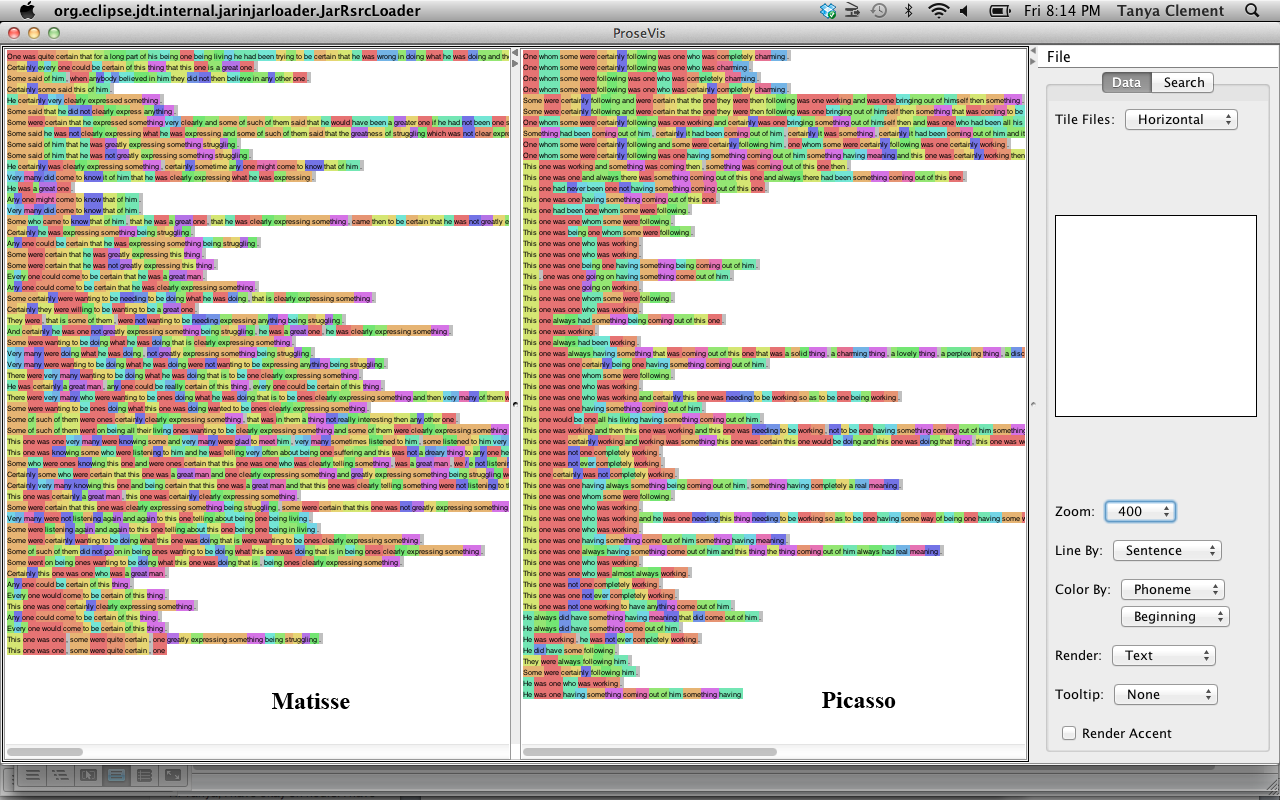
\includegraphics[scale=0.24]{../img/prosevis.png}
	\caption[Comparison of two poems in ProseVis]{Comparison of two poems in ProseVis. Reproduced from \cite{prosevis2017sourceforge}.}\label{screenshotProsevis}
\end{figure}

\subsection{Poemage and RhymeDesign}
Poemage (\cite{McCurdy2015poemage}) and RhymeDesign (\cite{McCurdy2015}) are both open-source applications with focus on analysis of sonic devices and sonic topology in poetry. Poemage\footnote{\url{http://www.sci.utah.edu/~nmccurdy/Poemage/}} focuses on complex structures of words connected through some sonic or linguistic resemblance across the space of the poem. It is available for MacOS or Windows with a web version currently under development. In MacOS application RhymeDesign -- which also provides the backend for Poemage -- users can enter their poem and query for one of the default rhyme types or choose a custom rhyme type.

\begin{figure}[h]\centering
	\includegraphics[scale=0.24]{../img/poemage.pdf}
	\caption{An example analysis in Poemage.}\label{screenshotPoemage}
\end{figure}

\subsection{Ambiances}
This software is unique in the fact that the analysis is integrated in the process of writing. As described in the paper \cite{Meneses2015}, writers enter the poem, receive a visualization and can control this visualization with body and hand gestures which in turn influence the poem. By such interconnection the authors aim to make Ambiances a part of the writing process and give it a chance to influence the final result. However, the actual software does not seem to be openly available.


\section{Generation tools}
\cite{lau2018deep} - learns rhyme automatically, for sonnets, results indistinguishable, apart from expert evaluation, missing emotion
\todo[inline]{generation by Reddy}
\todo[inline]{    - related work - generovani
	- deepspeare - ako oni generuju
	- gpt2
	- pravidlove generatory - tym sa nebudeme venovat, spomenut priklad}
\chapter{About data}
\chapter{Lyrics evaluation}
\todo[inline]{sucast zadania ze to bude bez zvukovej stranky hoci to vplyv ma}
\todo[inline]{pri popise taggeru dat typy rymov, ktore nezvlada}
\section{Rhyme detection}
\todo[inline]{Describe the original attempt with SPARSAR.- uviest priklady pesnicky, ktora sa zjavne rymuje ale urcilo ju to zle; priklad slova na ktorom sparsar spadne }

\subsection{Pronunciation}
\todo[inline]{spomenut ze nevieme zistit ci to spevak nevyslovi inak ,ze moze hltat bezprizvucne slabiky viac naraz
}

Unlike many other languages, English does not have a straightforward pronunciation rules. Therefore to be able to assess rhymes, we need to transcribe our text into a phonetic alphabet first. There are two commonly used alphabets to choose from -- IPA and ARPAbet. The original International Phonetic Alphabet (IPA) used since 1888 uses one UNICODE character to encode each phoneme and it is commonly used for example in dictionaries. Since it uses non-ASCII characters, ARPAbet was developed as an equivalent for computers. It has two versions: 1-character that uses upper-case and lower-case letters and 2-character version where each phoneme is represented by one or more upper-case ASCII characters (\cite{lea1980trends})(see Table\ref{pronunciation_table} for comparison). We will be using the 2-character ARPAbet because it is used by the CMUdict.

\begin{table}[h!]
	\centering
	\begin{tabular}{c c c c} 
		Example word & IPA & 1-character ARPAbet & 2-character ARPAbet \\ [0.5ex] 
		\hline
		st\textbf{o}ry & \textipa{O} & c & AO \\ 
		bu\textbf{tt}er & \textipa{R} & F & DX \\
	\end{tabular}
	\caption{Comparison of different pronunciation alphabets.}
	\label{pronunciation_table}
\end{table}

Carnegie Mellon University Pronouncing Dictionary (CMUdict) is an open-source pronunciation dictionary.\footnote{\url{http://www.speech.cs.cmu.edu/cgi-bin/cmudict}} Currently it contains 134,373 words (including their inflections) and their pronunciations in 2-character ARPAbet. 
For each word, there is one or several possible pronunciations in North American English including stress markers for primary, secondary or no stress. For the implementation, we used its Python wrapper package \textit{cmudict} \footnote{\url{https://pypi.org/project/cmudict/}}. To use this we need to strip the input of punctuation and convert it to lower case.

CMUdict is a large dictionary and it includes also slang words so it should cover most of our input. To test this, we looked at all last words on each line of our data (since those are the important ones for rhyme analysis) and we found out that 5.52\% of them are not in CMU dictionary. These included:

\begin{itemize}
	\item uncommon words, e.g. superglue, redundantly
	\item misspelled words, e.g. decsion, girlfren
	\item numbers
	\item foreign words, e.g. revoluccion, ecolli
	\item interjections and onomatopoeia, e.g. shoooshooo, woahwoah
\end{itemize}

Also, we applied some further data preprocessing that ensured more words in data would be found in the dictionary. We replaced the closing quotation mark "’" with the typewriter apostrophe "'" since only the second variant of apostrophe is accepted by CMUdict. We replaced hyphen "-" with a space " " to separate the hyphen-connected compound words into individual component words that have a higher chance of being found in the dictionary than the full version.
\todo[inline]{Describe here how we dealt with the ones not in CMUdict. Open MaryTTS?}

\subsection{Syllabification}
Once we have the pronunciations, we can start to compare them. When comparing lines for rhymes, we have to establish a system of alignment so that we analyze only relevant pairs of phonemes. Initially, we created a simple rhyme detector that just traversed both verses backwards phoneme by phoneme and compared them. However, rhyming words do not have to have an equal number of phonemes. For example words in the Table \ref{phon_misalign_table} have a 2-syllable rhyme. However if we compared each phonemes one by one they get misaligned on consonant clusters S-T-R and P-L and we will miss the second syllable rhyme.

\begin{table}[h!]
		\centering
	\begin{tabular}{c r} 
		Word & ARPAbet transcription \\ [0.5ex] 
		\hline
		constrain & K AH N - S T R EY N \\ 
		complain & K AH M - \space\space\space P L EY N \\
	\end{tabular}
	\caption{Example of misalignment when aligning by phonemes.}
	\label{phon_misalign_table}
\end{table}

We need to make sure that we are comparing corresponding parts of verses otherwise we will miss the rhyme. A better approach would be to compare corresponding syllables. Each syllable can be further split into 3 groups ("CVC") -- leading consonant cluster, vowel, and trailing consonant cluster. Consonant clusters can sometimes be empty. For syllabification we used python library \textit{syllabify} \footnote{\url{https://github.com/kylebgorman/syllabify}} which conveniently returns syllables in CVC triplets as described above.


\subsection{Calculating rating for one rhyme}
Finally, we have extracted pronunciation and syllables so we can continue to analyze the rhyme and rate the song. We decided to first calculate ratings for pairs of verses and then create an overall song rating based on these individual ratings. Another approach would be to analyze the complex statistics of the entire song and rate it at the end all at once. The second method could be better at incorporating the high-level properties like repeating of the refrain. We chose the first approach because it is more straight-forward and gives us a number for each rhyme which can be more interesting for the writer. Additional high-level analysis can be added later if necessary.

So let's focus on the rhyme analysis of two verses -- or rhyme fellows -- as they are typically called. Rhymes are located at the end of each line so there is no need to analyze the entire verse. How far should we look? The first choice would be to look at the last word. However rhymes can extend over more words as we see in \todo[inline]{Find an example of multi-word rhyme where the second word is unaccented}. When we look at the rhyme types, the basic ones do not go further then the first stressed syllable (looking at the line backwards). Notably, even if the rhyme does extend further we can ignore the rest because it will not contribute to the rating. According to our research, the most perfect rhyme is perfect rhyme so it should get the perfect score. And if there are more rhyming syllables preceding the perfect rhyme, they cannot make the score better. Similarly, if the rhyme is not perfect, syllables preceding the final stress would already be considered an internal rhyme -- which is also used (mainly in rap lyrics) but less valued than the classical end rhyme. We will therefore limit our window to the minimum number of syllables needed to include the stressed syllable in both rhyme fellows. Having a sequence of four unstressed syllables is very unlikely in English language so we limited our word preprocessing (pronunciation + syllabification) to last 4 syllables to speed up the performance.

To determine the rhyme we need to assess the match in sound of individual phonemes. Since we have each syllable separated into three groups we decided to give each group a number between -1 and 1 that would represent how similarly they sound. The numbers are assigned according to following heuristic:
\todo[inline]{Rewrite this list in a better-readable manner.}
\begin{itemize}
	\item 1 -- all phonemes are identical
	\item 0.75
	\begin{itemize}
		\item one is a subset of another
		\item it is a pair of similar sounding phonemes
	\end{itemize}
	\item A number between 0 and 1 if both are consonant clusters. This number is calculated:
	\begin{enumerate}
		\item Add 1/(length of the shorter consonant cluster) for each \textbf{shared} sound at the beginning or the end of the consonant clusters.
		\item Add 0.75/(length of the shorter consonant cluster) for each \textbf{similar} sound at the beginning or the end of the consonant clusters.
	\end{enumerate}
	\item 0 -- both are empty
	\item -0.5 -- one of them is empty
	\item -1 -- otherwise, meaning no matching or similar sounds
	
\end{itemize}

For an example of similarity evaluation see Table \ref{similarity_eval_table}.

\begin{table}[h!]
	\centering
	\begin{tabular}{c | c c c c} 
		$1^{st}$ verse & on & her & front & door \\ [0.5ex] 
		$2^{nd}$ verse & the & pain & no & more \\ 
		\hline
		$1^{st}$ pronunciation & \_, AA, N & HH, ER, \_ & F R, AH, N T & D, AO, R \\
		$2^{nd}$ pronunciation & DH, AH, \_ & P, EY, N & N, OW, \_ & M, AO, R \\
		\hline
		similarity & -0.5, 0.75, -0.5 & -1, -1, -0.5 & -1, -1, -0.5 & -1, 1, 1 \\
	\end{tabular}
	\caption{Example similarity evaluation for the last 4 syllables of two verses from song Cheatin' Woman by Lynyrd Skynyrd.}
	\label{similarity_eval_table}
\end{table}

To identify similar sounds, we look them up if there is a similarity group containing both of them. These similarity groups were created... \todo[inline]{Describe how it was done. The iterative approach? Or maybe Holtman's hierarchy? panPhon? \cite{mortensen2016panphon}}

Words for which we have not found pronunciation cannot be further processed so they are given rhyme rating 0 and skipped. Some words may have multiple possible pronunciations -- in that case we evaluate each possible combination of pronunciations for given line pair. After we assign a rating for each combination, we will keep only the best rated combination of pronunciations and discard the rest. 


With these similarity values we can proceed to calculate the rating which we decided to be as typically between 0 and 1. We will look at it syllable by syllable a return an average. There are some cases we need to consider individually:

\begin{itemize}
	\item different -- if all similarities are equal to -1, we can definitely say they do not rhyme and return a rating of 0
	\item identical -- since identity is a weaker rhyme than perfect, it will be given a penalty for "little creativity" returning a fixed rating of 0.8
	\item perfect -- perfect rhyme has a specific structure and if that holds, we can return the perfect score of 1.0 
\end{itemize}

For the remaining cases we will create rules based on how rhymes behave. Not all phonemes are equally important so let's assign weights to reflect it. The key role in rhyming plays the vowel so it should have the strongest impact on the rating. Second important is the ending consonant because it is closer to the end. Beginning consonant can add up to a nicer rhyme but it cannot bear the rhyme on its own. Since the vowel itself can be enough to create the rhyming effect it should have more weight than the rest combined. Therefore we assigned weights as follows:

Beginning consonants: 1,
Vowel: 4,
Ending consonants: 2

The rating for one syllable is created as normalized sum of weights times similarities. Furthermore, we need to account for stress. We can do that by multiplying the result with a multiplication factor depending on how does the stress match.

\begin{itemize}
	\item 1.0 for stressed rhyme because it is the strongest
	
	\item 0.9 for unstressed rhyme -- it is weaker but the stress pattern matches
	
	\item 0.8 for an mismatching stress pattern
\end{itemize}


The final formula for a rhyme rating is an average of syllable ratings and looks like this:

\[average(stress\_multiplication\_factor*weighted\_average(similarities))\]

\todo[inline]{This formula formatting looks weird but I don't have an idea how to do it better.}

\subsection{Calculating song rating}
\todo[inline]{rating celej piesne je priemer 2. stlpca, okrem '-' }
\todo[inline]{- rozlišovat terminologicky:
	- (rhyme) rating, tedy rating dvou veršů=řádků, číslo mezi 0 a 1
	- assigned (rhyme) rating, tedy rating, který nakonec danému řádku přidělíte(zatím jako nejvyšší možný z předchozích 1-5 řádků; případně 0, jsou-li všechny ratingy <0.8; případně žádný, jde-li o první řádku skupiny)
	- (rhyme) score, skóre celé písně, tedy průměr všech assigned ratings.}

The next step is to combine these rhyme ratings into one final rating for the entire song. In the previous section we created a function that returns rhyme rating for given two verses. To search for rhymes in the full lyrics we need to decide which verse pairs to check. The most straight-forward approach would be "brute force" -- try each line with all the other lines. Besides its obvious disadvantage of increased time requirements it also detects rhymes that span across tens of lines. It is not strictly defined how many lines apart can the rhyme fellows be to still be considered a rhyme -- the author can even make it a part of his artistic expression  e.g. in "Author's Prologue" by \cite{thomas1952author} the 1\textsuperscript{st} line rhymes with 102\textsuperscript{th}, 2\textsuperscript{nd} with 101\textsuperscript{th} and so on. But realistically, a rhyme between a line at the beginning of the lyrics and 20 lines later would not have an effect on the song listener -- it requires a close proximity of rhyme fellows within the poem. Since the most common stanzaic form in English is a quatrain, a stanza of four lines (\cite{eastman1970norton}), we decided to set the distance to 3. Further than that the effect on the reader gets weaker really fast. 
\todo[inline]{This probably needs a citation but I can't find any.}

As we decided, for each line, we will look at 3 preceding lines to look for its rhyme fellow. In case multiple of them rhyme, the one with the smallest distance will be selected -- if it is closer it is more probable the reader will associate it with the rhyme in the next line because it is the strongest in the memory. Consequently, a rating representing the score of this rhyming pair will be saved for the second rhyme fellow. It will not be saved for the first to ensure it will not be added to the final rating twice. The first of the pair will either keep a rating it shares with another line before or it will get an "X" (as seen in Table \ref{twinkle_analysis_table}) that represent no rating. 

Let's focus now on the first four line marked with rhyme scheme letter "e" in Table \ref{twinkle_analysis_table}. They all rhyme with each other and all rhymes except for \textit{are/dark} are perfect. That means the line with "dark" would receive less than perfect score and it would lower the score of the entire song. If we instead ignore this rhyme and associate only the first two and the last two rhymes together we will receive a perfect score. Loosing rating by marking weaker rhymes does not make sense so we must add an exception to only keep the better score.

Using the ratings added to the lines a final score will be calculated as the average of lines that have a rating (not an "X").

\todo[inline]{Counterexample - we have a 4-line song where 2 lines rhyme and a 24-line song where 2 lines rhyme - they will receive the same score. That does not seem fair?}


 Rhymes in songs or poems are typically marked using a rhyme scheme. That means each verse gets assigned a letter -- lines that share the same letter rhyme and those with different letters do not. We also decided to adapt this common notation. In case the song needs more letters than there are in the alphabet we will add another letter and continue alphabetically -- aa, ab, ac, ..., ba, bb, bc, ..., ca, etc.


\begin{table}[h!]
	\centering
	\begin{tabular}{c|c|c|c} 
	Rhyme & Rating & Lyrics & \begin{tabular}{@{}c@{}}Pronunciation \\ (last 2 syllables)\end{tabular}  \\ 
	\hline
	\hline 
	a  & X    & Twinkle twinkle little star & 'T AH L', 'S T AA R' \\ 
	a  & 1.0  & How I wonder what you are & 'Y UW ', ' AA R' \\
	b  & X    & Up above the world so high & 'S OW ', 'HH AY ' \\
	b  & 1.0  & Like a diamond in the sky &  'DH AH ', 'S K AY ' \\
	a  & 1.0  & Twinkle twinkle little star & 'T AH L', 'S T AA R'\\
	a  & 1.0  & How I wonder what you are &  'Y UW ', ' AA R' \\ [0.5ex]
	\hline
	c  & X    & When the blazing sun is gone &  ' IH Z', 'G AO N' \\
	c  & 0.8  & When he nothing shines upon & ' AH ', 'P AA N' \\
	d  & X    & Then you show your little light & 'T AH L', 'L AY T' \\
	d  & 1.0  & Twinkle twinkle all the night &  'DH AH ', 'N AY T' \\
	e  & X    & Twinkle twinkle little star &  'T AH L', 'S T AA R' \\
	e  & 1.0  & How I wonder what you are &  'Y UW ', ' AA R' \\[0.5ex]
	\hline
	e  & X    & Then the traveler in the dark & 'DH AH ', 'D AA R K' \\
	e  & 1.0  & Thanks you for your tiny spark &  'N IY ', 'S P AA R K' \\
	f  & X    & He could not see which way to go &  'T UW ', 'G OW ' \\
	f  & 1.0  & If you did not twinkle so & 'K AH L', 'S OW ' \\
	e  & X    & Twinkle twinkle little star &  'T AH L', 'S T AA R' \\
	e  & 1.0  & How I wonder what you are &  'Y UW ', ' AA R' \\[0.5ex]
	\hline
	g  & X    & In the dark blue sky you keep & 'Y UW ', 'K IY P' \\
	g  & 1.0  & Often through my curtains peep &  'T AH N Z', 'P IY P' \\
	h  & X    & For you never shut your eye &  'Y AO R', ' AY ' \\
	h  & 1.0  & Till the sun is in the sky & 'DH AH ', 'S K AY ' \\
	i  & X    & Twinkle twinkle little star & 'T AH L', 'S T AA R' \\
	i  & 1.0  & How I wonder what you are &  'Y UW ', ' AA R' \\
	\end{tabular}
	\caption{Example of song analysis of the nursery rhyme "Twinkle, Twinkle Little Star" with a final rating of 0.989.}
	\label{twinkle_analysis_table}
\end{table}


	
\noindent\rule{14cm}{0.4pt}

Since meter plays an important role in rhymes, another relevant property to examine is the number of syllables. To count syllables for each line we used Python package \textit{syllabify} \footnote{\url{https://github.com/kylebgorman/syllabify}} which returns syllables using ARPAbet transcription. For words not in CMUdict we used a simple heuristic -- since the nucleus of each syllable is most often a vowel (except for syllabic consonants) we counted the number of (groups of) vowels and used it as an estimation for the number of syllables. Although this gives a wrong estimate for words like \textit{rhythm} or \textit{house}it performed quite well when we tested it on a few out-of-dictionary words from our dataset. We found it unnecessary to try to further improve the heuristic since the words that are not in CMUdict are often foreign words that do not follow the standard pronunciation rules of English so any application of these rules would probably be of little help.

\todo[inline]{Nemalo by tu mozno byt este nieco o tom ako sme to testovali? Resp. netreba to odtestovat nejak systematickejsie nez od oka?}

\chapter{Generation}\label{generation}
Writing a lyrics for a song is a task that requires creativity. This is one of a few areas where AI has not become better than humans yet. While it is generally capable of keeping similar structure and topic, it still fails use rhymes and other literary devices.

As described in section \ref{generation_tools}, current state-of-art tool for generation is GPT-3 \cite{brown2020gpt3}. We have sent several requests for their API but have not received a reply to this day.

The second-best option was its earlier version GPT-2 (\cite{radford2019gpt2}). It offers pre-trained models of sizes small, medium, large, and XL that can be further fine-tuned to the specific task. Since training models of such sizes has very high memory requirements, we would only be able to fine-tune the small model on available school clusters. 

However, our colleagues from UFAL institute at Charles University agreed to let us generate on GPT-2 XL that they are using in their ongoing research project THEaiTRE (\cite{rosa2021theaitre}). It is a vanilla model, meaning that it has not been fine-tuned to specific task and we do not have resources to fine-tune it. But as their research confirms, it is not necessary because it adapts very well when given a relevant primer. Knowing it has been trained on 8 million web pages, it is highly probable that it has already seen our data (or some similar web containing lyrics data). 

Without fine-tuning, the quality of the result depends on the selection of the primer. To choose what works the best, we decided to compare the results using primers of different lengths. For starters, we tried one-line primer. As expected, it was not enough for GPT-2 to recognize it as poetry, and it continued with full paragraph as you can see in Figure \ref{fig_1line_primer}.

\begin{figure}[htb]\centering
	\minipage{0.9\textwidth}
	A chair is still a chair \\
	\color{blue}In most other aspects, I think the two camps in this debate can agree. We're in good company, for instance, as far as the law is concerned. When it comes to the "should" part of the debate, the fact that some states have no-fault insurance mandates, and others have them, is not a matter of opinion, or of opinion alone. \\
	\endminipage\hfill
	\caption{Result of generation (in blue) using 1-line primer (in black).} \label{fig_1line_primer}
\end{figure} 

Subsequently, we iteratively increased the length of the primer exponentially. We conducted experiments with several song lyrics, but the results did not differ very much, so we show one example in Table \ref{generation_result}.

Except for the 4-line primer, it was able to successfully replicate the poem-like structure. It also used a lot of repetition, even when the original text did not contain any (e.g. 2-line primer). We assume, it must have already learned that repetition is very common for this text structures. However, it was not successful in creating rhymes of its own. 

Although longer primer seems to be a safer path to good result, it does not seem to be significantly better than the result from 2-line primer. Occasionally, it appears to miss the clue and continue with regular text, as it did with 4-line primer here.

%"url": "http://genius.com/Luther-vandross-a-house-is-not-a-home-lyrics", "year": "1981-08-12", "lang": "en", "id": 13056, "word_count": 310,

\begin{table}[!h]
	\begin{tabular}{cc}
		\textbf{Original} &   \textbf{2-line primer} \\ \midrule
			\begin{minipage}[t]{0.47\textwidth}
		A chair is still a chair\\
		Even when there's no one sittin' there\\
		But a chair is not a house\\
		And a house is not a home\\
		When there's no one there to hold you tight\\
		And no one there you can kiss goodnight\\
		Woah girl
		\end{minipage}
		 & 
		\begin{minipage}[t]{0.47\textwidth}
		A chair is still a chair\\
		 Even when there's no one sittin' there\\
		 \color{blue} I still think there are people here\\
		 A chair is still a chair\\
		 Even when there's no one sittin' thereI still think there are people here\\
		 A chair is still a chair 
		 \end{minipage}\\[6pt]
	 \textbf{4-line primer} &   \textbf{8-line primer} \\ \midrule
	 \begin{minipage}[t]{0.47\textwidth}
	 	A chair is still a chair\\
	 	Even when there's no one sittin' there\\
	 	But a chair is not a house\\
	 	And a house is not a home\\
		\color{blue}
	 	So why do we make up the terms?\\
	 	It's not just us who insist on the word house, we use it in all sorts of other contexts too. For example, if you want to use a single word to refer to a group of people, you might say:\\
	 	If you want to invite everyone to an event, you might say:\\
	 	It's not hard to see why we seem to love using a term like 'house' to refer to a group of people – it's the easiest word for us to remember.
	 \end{minipage}
	 & 
	 \begin{minipage}[t]{0.47\textwidth}
	 A chair is still a chair\\
	 Even when there's no one sittin' there\\
	 But a chair is not a house\\
	 And a house is not a home\\
	 When there's no one there to hold you tight\\
	 And no one there you can kiss goodnight\\
	 Woah girl\\
	 \\
	 A room is a still a room\\
	 \color{blue} And a still a room is still a home\\
	 When there's no one there to hold you tight\\
	 And no one there you can kiss goodnight\\
	 I'm a little man on a little island\\
	 And a lonely little bird on a lonely little island\\	 
	 But a lonely little bird is not a castle\\
	 And a lonely little bird is not a home\\
	 And a lonely little bird is not a world\\
	 I'm a little man in a little house\\
	 And a lonely little bird in a lonely little house
	 \end{minipage}\\[6pt]
	\end{tabular}
	\caption{Beginning of "A House Is Not A Home" lyrics by Luther Vandross. Comparison with results generated using 2,4, and 8-line primers.}
	\label{generation_result}
\end{table}

%Clouds Crash Lyrics by The matches, pop

Overall, GPT-2 succeeded in replicating the poetic form and structure. It creatively generated meaningful content that was very close to human-written. A slight give-away is excessive repetition, but for an individual example, could be mistaken for author's style.



\chapter*{Conclusion}
\addcontentsline{toc}{chapter}{Conclusion}


%%% Bibliography
%%% Bibliography (literature used as a source)
%%%
%%% We employ bibTeX to construct the bibliography. It processes
%%% citations in the text (e.g., the \cite{...} macro) and looks up
%%% relevant entries in the bibliography.bib file.
%%%
%%% The \bibliographystyle command selects, which style will be used
%%% for references from the text. The argument in curly brackets is
%%% the name of the corresponding style file (*.bst). Both styles
%%% mentioned in this template are included in LaTeX distributions.

\bibliographystyle{plainnat}    %% Author (year)
% \bibliographystyle{unsrt}     %% [number]

\renewcommand{\bibname}{Bibliography}

%%% Generate the bibliography. Beware that if you cited no works,
%%% the empty list will be omitted completely.

\bibliography{bibliography}

%%% If case you prefer to write the bibliography manually (without bibTeX),
%%% you can use the following. Please follow the ISO 690 standard and
%%% citation conventions of your field of research.

% \begin{thebibliography}{99}
%
% \bibitem{lamport94}
%   {\sc Lamport,} Leslie.
%   \emph{\LaTeX: A Document Preparation System}.
%   2nd edition.
%   Massachusetts: Addison Wesley, 1994.
%   ISBN 0-201-52983-1.
%
% \end{thebibliography}


%%% Figures used in the thesis (consider if this is needed)
\listoffigures

%%% Tables used in the thesis (consider if this is needed)
%%% In mathematical theses, it could be better to move the list of tables to the beginning of the thesis.
\listoftables

%%% Abbreviations used in the thesis, if any, including their explanation
%%% In mathematical theses, it could be better to move the list of abbreviations to the beginning of the thesis.
\clearpage
\printglossary[title=Glossary of literary  and technical terms]

%%% Attachments to the master thesis, if any. Each attachment must be
%%% referred to at least once from the text of the thesis. Attachments
%%% are numbered.
%%%
%%% The printed version should preferably contain attachments, which can be
%%% read (additional tables and charts, supplementary text, examples of
%%% program output, etc.). The electronic version is more suited for attachments
%%% which will likely be used in an electronic form rather than read (program
%%% source code, data files, interactive charts, etc.). Electronic attachments
%%% should be uploaded to SIS and optionally also included in the thesis on a~CD/DVD.
%%% Allowed file formats are specified in provision of the rector no. 72/2017.
\appendix
\chapter{Attachments}

Following tables show the transcription between IPA and ARPAbet for vowels (Figure \ref{ipa-arpa-vowels}) and consonants (Figure \ref{ipa-arpa-cons}). Note, that IPA diphthongs are not transcribed separately but as one two-character ARPAbet symbol.

\begin{table}[h!]
	\centering
	\begin{tabular}{c c c} 
		ARPAbet & IPA & Example \\ [0.5ex] 
		\hline
		AA  &\textipa{A}	&balm, bot \\
		AE	&æ	&bat	\\
		AH	&\textipa{2}	&butt	\\
		AO	&\textipa{O}	&story	\\
		AW	&\textipa{aU}	&bout	\\
		AX	&\textipa{@}	&comma	\\
		AXR	&\textipa{@r}	&letter\\
		AY	&\textipa{aI}	&bite	\\	
		EH	&\textipa{E/e}	&bet	\\
		ER	&\textipa{3r}	&bird	\\
		EY	&\textipa{eI}	&bait	\\
		IH	&\textipa{I}	&bit	\\
		IX	&\textipa{1/---}	&roses, rabbit\\
		IY	&i	&beat	\\
		OW	&\textipa{oU}	&boat	\\
		OY	&\textipa{OI}	&boy	\\
		UH	&\textipa{U}	&book	\\
		UW	&u	&boot	\\
		UX	&\textipa{0/---}	&dude\\
	\end{tabular}
	\caption{Vowel phonemes - transcription between IPA and ARPAbet.}
	\label{ipa-arpa-vowels}
\end{table}


\begin{table}[h!]
	\centering
	\begin{tabular}{c c c} 
		ARPAbet & IPA & Example \\ [0.5ex] 
		\hline
		
	\end{tabular}
	\caption{Consonant phonemes - transcription between IPA and ARPAbet.}
	\label{ipa-arpa-cons}
\end{table}



\openright
\end{document}
